\documentclass[a4paper,12pt,preview]{report} %размер бумаги устанавливаем А4, шрифт 12пунктов
\usepackage[english,russian]{babel}%используем русский и английский языки с переносами 	
\usepackage[T2A]{fontenc}
\usepackage{changepage}
\usepackage{lipsum}
\usepackage{indentfirst}
\usepackage[labelsep=period]{caption}
\usepackage{amsmath}
\usepackage[utf8]{inputenc}%включаем свою кодировку: koi8-r или utf8 в UNIX, cp1251 в Windows
\usepackage[english,russian]{babel}%используем русский и английский языки с переносами 	
\usepackage{amssymb,amsfonts,amsmath,mathtext,cite,enumerate,float} %подключаем нужные пакеты расширений
\usepackage{graphicx} %хотим вставлять в диплом рисунки?
\usepackage{indentfirst}
\usepackage{titlesec}
\graphicspath{{images/}}%п\usepackage{trd}уть к рисункам
\usepackage{hyperref}
\hypersetup{
	colorlinks,
	citecolor=black,
	filecolor=black,
	linkcolor=black,
	urlcolor=black
}

\makeatletter
\renewcommand{\@biblabel}[1]{#1.} % Заменяем библиографию с квадратных скобок на точку:
\makeatother

\usepackage{geometry} % Меняем поля страницы
\geometry{left=2cm}% левое поле
\geometry{right=1.5cm}% правое поле
\geometry{top=1cm}% верхнее поле
\geometry{bottom=2cm}% нижнее поле

\renewcommand{\theenumi}{\arabic{enumi}}% Меняем везде перечисления на цифра.цифра
\renewcommand{\labelenumi}{\arabic{enumi}}% Меняем везде перечисления на цифра.цифра
\renewcommand{\theenumii}{.\arabic{enumii}}% Меняем везде перечисления на цифра.цифра
\renewcommand{\labelenumii}{\arabic{enumi}.\arabic{enumii}.}% Меняем везде перечисления на цифра.цифра
\renewcommand{\theenumiii}{.\arabic{enumiii}}% Меняем везде перечисления на цифра.цифра
\renewcommand{\labelenumiii}{\arabic{enumi}.\arabic{enumii}.\arabic{enumiii}.}% Меняем везде перечисления на цифра.цифра

\newcommand{\doublerule}[1][.4pt]{%
	\noindent
	\makebox[0pt][l]{\rule[.7ex]{\linewidth}{#1}}%
	\rule[.3ex]{\linewidth}{#1}}



%\titleformat{\chapter}{}{}{0em}{\bfseries\LARGE\ifnum\value{chapter}>0\ifnum\value{chapter}<3\relax\arabic{chapter}.~\fi\fi}
\titleformat{\chapter}[hang]
{\normalfont\huge\bfseries}{\thechapter.}{20pt}{}


\begin{document}
	В последнее время общее количество обращений клиентов банков по продуктам очень сильно возросло. В банковской среде возникает потребность в решении задачи \textit{поиска корневой причины} обращений. В настоящее время эта задача решается вручную или полуавтоматически.
	
	Целью этой работы ставится создание полностью автоматической системы, так как это приведет к уменьшению расходов на штат и увеличит качество предоставления услуг.
	
	\begin{center}
	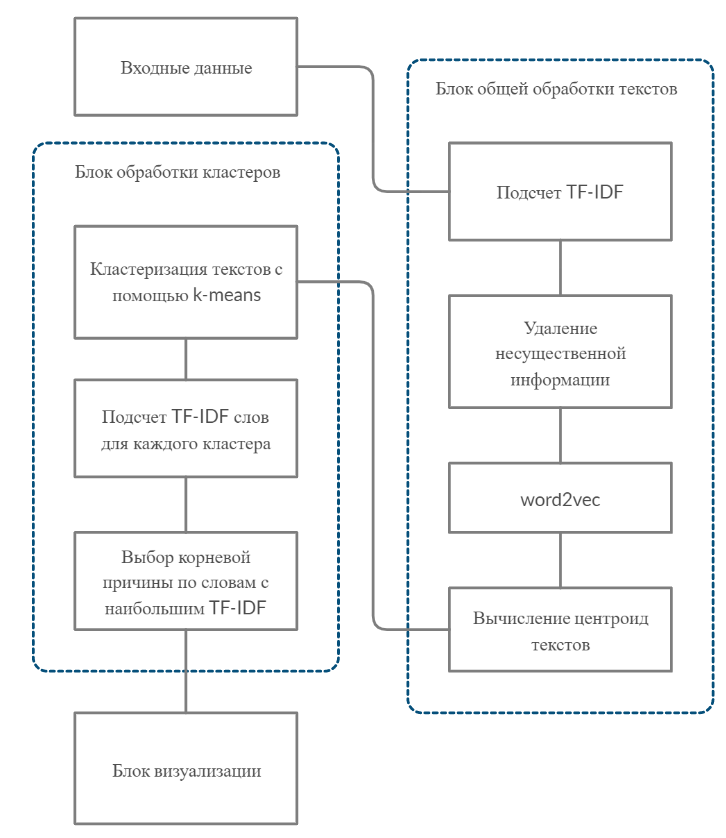
\includegraphics[scale=0.5]{SCHEME.png}
	
	Рис. 1. Функциональная схема работы
	\end{center}
	
	Автором предложен следующий алгоритм решения задачи: для начала нужно произвести нормализацию исходных данных, то есть приведения текста обращения в нормальную (словарную) форму. Это нужно для того, чтобы одно слово в разных словарных формах (например, падежах) считалось системой за одну и ту же смысловую единицу. Далее считается их характеристика TF-IDF, далее удаляются слова с самым низким и самым высоким показателем TF-IDF, так как установлено, что таковые очень часто являются несущественными. Далее слова преобразуются в вектора с помощью word2vec, эти векторы будут отображать эмбеддинги (смыслы) слов. После этого по векторам вычисляется центроиды текстов, к которым применяется алгоритм k-means для кластеризации по корневым причинам. Для каждого кластера снова считается TF-IDF слов. Несколько (2-5) слов с наибольшим TF-IDF выбираются в качестве корневой причины. Также предусмотрена визуализация для мониторинга основных корневых причин.	
	
	Алгоритм реализован на языке программирования Python3, с помощью модулей Pymorphy2, nltk и gensim. В данный момент разработка находится на стадии тестирования и получения численных оценок качества работы.
	
	
	
\end{document}

